%\documentclass{class-for-drafts}
\documentclass[a4paper,english]{lipics-v2016}

\usepackage{hyperref}
%% url
\usepackage{url}
%% maths
\usepackage{amsmath,amssymb,bm}
%%\usepackage{amsfonts}
%% \usepackage{amsthm}
%% algorithms
%\usepackage{algorithm}
\usepackage{algorithmicx}
%\usepackage[noend]{algpseudocode}
\usepackage[ruled, linesnumbered, noend]{algorithm2e}
\usepackage{multicol}

\usepackage{pifont}

%% images
\usepackage{graphicx}
%\usepackage[dvipsnames]{xcolor}
%% inparaenum
\usepackage{paralist}
\usepackage{enumitem}
%% tables
\usepackage{booktabs,multirow,tabularx,hhline}
\usepackage{makecell}
%% figures
%\usepackage{caption}
%\usepackage{subfig}
%\usepackage[font=small, skip=2pt]{caption}
%\usepackage[font=small]{subfig}
\usepackage{tikz}
\usetikzlibrary{arrows.meta,decorations.pathreplacing,decorations.pathmorphing,plotmarks,shapes,matrix,patterns}
\usepackage[normalem]{ulem}
\tikzset{>={Latex[width=3pt,length=5pt]}}
%% transform eps in pdf crossplateform
\usepackage{epsfig}
\usepackage{epstopdf}

%% hyphenation
\usepackage{hyphenat}
\hyphenation{brow-sers brow-ser}

\newcommand{\TODO}[1]{\textcolor{red}{#1}}
\newcommand{\REF}[0]{\textcolor{purple}{REF}}
\newcommand{\COLOR}[2]{\textcolor{#1}{#2}}

\usepackage{xspace}
\newcommand{\SCAMP}[0]{\textsc{Scamp}\xspace}
\newcommand{\CYCLON}[0]{\textsc{Cyclon}\xspace}
\newcommand{\SPRAY}[0]{\textsc{Spray}\xspace}
\newcommand{\LSEQ}[0]{\textsc{LSeq}\xspace}
\newcommand{\CRATE}[0]{\textsc{Crate}\xspace}
\newcommand{\PEERSIM}[0]{\textsc{PeerSim}\xspace}

\newcommand{\PCBROADCAST}[0]{\textup{PC-broadcast}\xspace}
\newcommand{\RPCBROADCAST}[0]{\textup{RPC-broadcast}\xspace}

\usepackage{amsthm} %% proof env
%\newtheorem{definition}{Definition}
%\newtheorem{theorem}{Theorem}
%\newtheorem{lemma}{Lemma}
\newtheorem*{problem*}{Problem statement}

\newcommand{\EXAMPLE}[2]{\noindent \textbf{\emph{#1}} #2}
\newcommand{\PAR}[2]{\noindent \textbf{#1} #2}

%%%%%%%%%%%%%%%%%%%%%%%%%%%%%%%%%%%%%%%%%%%%%%%%%%%%%%%%%%%%%%%%%%%%%%%%%%%%%%%
%%%%%%%%%%%%%%%%%%%%%%%%%%%%%%%%%%%%%%%%%%%%%%%%%%%%%%%%%%%%%%%%%%%%%%%%%%%%%%%
%%%%%%%%%%%%%%%%%%%%%%%%%%%%%%%%%%%%%%%%%%%%%%%%%%%%%%%%%%%%%%%%%%%%%%%%%%%%%%%

\begin{document} 

\title{The Last Linear Upper Bound of Causal Broadcast}

%\numberOfAuthors{1}

\newcommand{\affLSNN}{LS2N, University of Nantes\\
   2 rue de la Houssini{\`e}re\\
   BP 92208, 44322 Nantes Cedex 3, France}
%   \url{first.last@univ-nantes.fr}}

\author[1]{Brice N{\'e}delec}
\author[2]{Pascal Molli}
\author[3]{Achour Most{\'e}faoui}
\affil[1]{\affLSNN\\\url{brice.nedelec@univ-nantes.fr}}
\affil[2]{\affLSNN\\\url{pascal.molli@univ-nantes.fr}}
\affil[3]{\affLSNN\\\url{achour.mostefaoui@univ-nantes.fr}}
\authorrunning{B. N{\'e}delec, P. Molli and A. Most{\'e}faoui}
%\proceedings{}

\keywords{Causal broadcast, reliable broadcast, space complexity, large and dynamic
distributed systems}

\subjclass{C.2 Computer-communication networks}

\Copyright{Brice N{\'e}delec, Pascal Molli and Achour Most{\'e}faoui}

\maketitle


\IEEEtitleabstractindextext{
\begin{abstract}
  Causal broadcast constitutes the fundamental communication primitive of many
  distributed protocols and applications. However, state-of-the-art
  implementations do not scale in large and dynamic systems.  In this paper, we
  propose a novel implementation of causal broadcast. Message overhead is
  constant. Local space complexity is non-monotonic and depends on system
  settings and current usage. We prove that all and only obsolete control
  information is discarded, at the cost of few lightweight control messages.
  Our implementation constitutes a better and sustainable communication
  primitive for causal broadcast in large and dynamic systems.
\end{abstract}
}

% \begin{abstract}
%   Causal broadcast constitutes the core communication primitive of many
%   distributed systems. For decades, state-of-the-art approaches relied on
%   maintaining and transmitting vector clocks. The size of vector clocks
%   increases linearly with the number of processes that ever entered the
%   system. Causal broadcast eventually became overcostly and inefficient in large
%   and dynamic systems.  A recent approach solved the issue about generated
%   traffic by removing the need for transmitting vectors. However, it still
%   maintains a vector locally. In this paper, we improve this causal broadcast by
%   removing the need for such vector. The proposed protocol safely purges the
%   local structure over time at cost of few control messages. As consequence,
%   causal broadcast can run in large and dynamic systems even on most humble
%   devices such as Raspberry Pi's.
% \end{abstract}

% \keywords{Causal broadcast, local space complexity}


%%% Local Variables:
%%% mode: latex
%%% TeX-master: "../paper"
%%% End:

 
\section{Introduction}

Causal broadcast constitutes the core communication primitive of many
distributed systems~\cite{hadzilacos1994modular}. Applications such as
distributed social networks~\cite{borthakur2013petabyte}, distributed
collaborative software~\cite{heinrich2012exploiting,nedelec2016crate}, or
distributed data
stores~\cite{bailis2013bolton,bravo2017saturn,demers1987epidemic,lloyd2011cops,shapiro2011comprehensive}
use causal broadcast to ensure consistency criteria.  Causal broadcast ensures
the reliable delivery of broadcast messages, exactly once, following Lamport's
happen before relationship~\cite{lamport1978time}. When Alice comments Bob's
picture, nobody sees Alice's comment without Bob's picture, and nobody sees
Alice's comment or Bob's picture multiple times.
% If the sending of a message $m$ precedes the sending of a message $m'$ then all
% processes that deliver these two messages need to deliver $m$ before
% $m'$. Otherwise they deliver them in any order.

In large and dynamic systems, processes cannot afford to maintain an up-to-date
knowledge of the full membership (\REF). Instead, each process builds a partial view of
neighbors to communicate with. Gossiping (\REF) exploits these neighborhoods to
efficiently broadcast a message to all processes. To broadcast a message, a
process sends the message to its neighbors; each process receiving such message
forwards it to its own neighbors. Processes receive the message either directly
or transitively. Processes may receive a broadcast message multiples times from
different sources.  To deliver each message exactly once, reliable broadcast
must discard the additional copies of the original message at receipt.

In static systems where processes cannot join, leave, or self-reconfigure their
neighborhood, the local structure that ensures exactly once delivery is
lightweight.  Since each process forwards each message exactly once, each
process knows that it will receive a number of copies of the original message
equal to the number of their incoming links. Once it received that many copies,
it safely purges its local structure from this message. It will never receive
this message again.  However, in dynamic systems, when a process adds a neighbor
to its partial view, the latter does not know if it should expect another
message copy from this new incoming link. It may cause multiple deliveries of a
same message.

To solve this, broadcast protocols maintain a summary of past delivered messages
(\REF). Upon receipt, processes quickly identify whether they should deliver the
message or discard it. However, the size of this structure increases linearly
with the number of processes that ever broadcast a message (\REF). This dampens
the usage of broadcast protocols. In particular, humble devices with limited
local memory cannot afford it, and reclaiming elements from the structure
requires an overcostly distributed consensus (\REF).

% \TODO{We do reliable broadcast on top of causal broadcast. Did not make sense
%   before because the cost of causal broadcast was too high. Now that it's cheap,
%   we use it to enable reliability at marginal cost.}

% State-of-the-art causal broadcasts (\REF) reuse this vector of clocks. Each
% message piggybacks such vector to ensure their causal delivery. A recent causal
% broadcast (\REF) alleviates processes from the need for piggybacking vectors in
% messages. However, it still requires to maintain the local vector to ensure that
% it delivers each message exactly once.

\begin{table}
  \begin{center}
    \caption{\label{table:complexity} Complexity of broadcast algorithms at each
      process. $N$ the number of processes that ever broadcast a message. $P$
      the number of processes in the system. $W$ the number of messages received
      but not delivered yet. $Q_i$ is the number of processes in the inview. $M$
      is the number of messages already delivered that should be received again
      from at least one process in $Q_i$.}
    \newcommand{\cmark}{\ding{51}}%
\newcommand{\xmark}{\ding{55}}%

\setlength{\tabcolsep}{4pt} % General space between cols (6pt standard)

\small

\begin{tabularx}{0.98\columnwidth}{@{}Xcccc@{}}
  & \makecell{message\\overhead} &  \makecell{delivery\\execution time} & \makecell{local space\\consumption} & \makecell{\# control messages\\per added link} \\ \cmidrule{2-5}
  reliable broadcast~\cite{hadzilacos1994modular} & $O(1)$ & $O(1)$ & $O(N)$ & $0$ \\
  vector-based causal broadcast~\cite{schwarz1994detecting} & $O(N)$ & $O(W.N)$ & $O(N+W.N)$ & $0$ \\ 
  \PCBROADCAST (\REF) & $O(1)$ & $O(1)$ & $O(N)$ & $3$ to $2P^2$ \\ \hline\hline
  \textbf{this paper (\RPCBROADCAST)} & $O(1)$ & $O(Q_i)$ & $\mathbf{O(Q_i.M)}$ & $\mathbf{6}$ to $\mathbf{4P^2}$ \\
%  \bottomrule
\end{tabularx}

%%% Local Variables:
%%% mode: latex
%%% TeX-master: "../paper"
%%% End:

  \end{center}
\end{table}

In this paper, we present a causal broadcast protocol that exploits causal order
to get rid of the summary of past delivered messages. 
%\TODO{Maybe more generic: on top of any causal broadcast? Along with
%  \PCBROADCAST it removes the last linear complexity?}
Our contribution is threefold:
\begin{itemize}[leftmargin=*]
\item We extend the causal broadcast protocol proposed in (\REF) to remove the
  last linear upper bound in terms of number of processes that ever broadcast a
  message that remains on local space complexity. Similarly to \REF, it only
  makes use of temporary buffers and few control messages to ensure both causal
  order and reliability. We provide the corresponding formal proof.
  % describe a causal broadcast that piggybacks constant size control information
  % while maintaining a local structure that is safely purged over time, and we
  % prove it.
\item We provide the complexity analysis of our causal broadcast
  protocol. Table~\ref{table:complexity} shows that removing the last linear
  upper bound $N$ cost twice as much in terms of number of control messages as
  ensuring causal order. Depending on the system (\REF), the number of messages
  stays close to its lower bound $6$. The local space consumption consists of
  buffers that grow and shrink in dynamic settings.
\item We provide experimentation highlighting the impact of our protocol on
  transmission delays before delivery and the generated traffic. \TODO{More.}
\end{itemize}
\RPCBROADCAST proposes an advantageous tradeoff that makes causal broadcast a
lightweight and efficient middleware in large and dynamic systems. This tradeoff
even makes \RPCBROADCAST a lightweight and efficient implementation of reliable
broadcast. By removing the last linearly and monotonically increasing structure,
these broadcast protocols can run in large and dynamic systems even on most
humble devices such as Raspberry Pi's. \TODO{It also makes scalable all
  protocols that rely on causal broadcast.}

The rest of this paper is organized as follows. Section~\ref{sec:motivations}
shows the issue and motivates this work. Section~\ref{sec:proposal} presents the
proposed causal broadcast and corresponding
proofs. Section~\ref{sec:experimentation} highlights the pros and cons of our
approach on experimental setups. We conclude in Section~\ref{sec:conclusion}.


%%% Local Variables:
%%% mode: latex
%%% TeX-master: "../paper"
%%% End:

%
\section{Issues and Motivations}
\label{sec:motivations}

Causal broadcast is a communication primitive that allows a process to send
messages to all processes of its distributed system. Message deliveries follow
the happen before relationship. If the sending of a message $m$ precedes the
sending of a message $m'$ then all processes that deliver these two messages
need to deliver $m$ before $m'$. Otherwise they deliver them in any order. Each
process may receive a message multiple times but it delivers it exactly once.

Causal broadcast relies on reliable broadcast. First, it guarantees that all
correct processes eventually receive broadcast messages. Gossiping constitutes
an efficient mean to reliably disseminate messages to large systems. Each
process maintains a partial view considerably smaller than the whole system
membership. When a process broadcasts a message, it sends it to its partial
view; each process that receives such message forwards it to its partial
view. Broadcast messages reach all processes either directly or transitively.

\begin{figure*}
  \begin{center}
    \subfloat[Part A][\label{fig:generalpurgeA}Process~A broadcasts $a$. It expects 
    two copies of $a$.]
    {\input{input/figgeneralpurgeA.tex}}
    \hspace{10pt}
    \subfloat[Part B][\label{fig:generalpurgeB}Process~B and Process~C receive
    and deliver $a$. They both expect an additional copy of $a$.]
    {\input{input/figgeneralpurgeB.tex}}
    \\
    \subfloat[Part C][\label{fig:generalpurgeC}Process~B and Process~C forward $a$ 
    to their neighbors in a gossip fashion.]
    {\input{input/figgeneralpurgeC.tex}}
    \hspace{10pt}
    \subfloat[Part D][\label{fig:generalpurgeD}All processes receive a copy
    of $a$. Process~B and Process~C do not expect additionnal copies of $a$. 
    Process~A still expects a copy.]
    {\input{input/figgeneralpurgeD.tex}}
    \\
    \subfloat[Part E][\label{fig:generalpurgeE}Process~A receives the last 
    awaited copy of $a$. It purges its structure from this message.]
    {\input{input/figgeneralpurgeE.tex}}
    \caption{\label{fig:generalpurge}Broadcast that guarantees to deliver 
      messages exactly once using counters.}
  \end{center}
\end{figure*}


Second, reliable broadcast guarantees that each process delivers each broadcast
message exactly once, in spite of multiple receipts that can occur.
Figure~\ref{fig:generalpurge} shows a lightweight implementation that consists
in recording the number of copies expected after the first receipt. When the
expected number of copies falls to zero, the message will never be received
again. Reliable broadcast purges its local structure from this element. In
Figure~\ref{fig:generalpurgeA}, Process~A broadcasts $a$ to Process~B and
Process~C. Since it knows that each process forwards each message exactly once,
it expects to receive 2 copies: one from Process~B, one from Process~C. In
Figure~\ref{fig:generalpurgeB}, Process~B and Process~C receive and deliver
$a$. They both expect another copy of $a$ from Process~C and Process~B
respectively. Since this is their first receipt of $a$, Process~B and Process~C
forward the message to their neighbors. In Figure~\ref{fig:generalpurgeD},
Process~B and Process~C receives the awaited copy from each other. They will
never receive such message again, so they remove it from the set of expected
messages. Process~A receives a copy but does not purge its local structure, for
it still expect an additional copy of the message. It decrements the counter
corresponding to $a$. In Figure~\ref{fig:generalpurgeE}, Process~A finally
receives the last copy of $a$ and purges its structure.

\begin{figure*}
  \begin{center}
    \subfloat[Part A][\label{fig:generalproblemA}Process~A broadcasts $a$. It expects 
    two copies of $a$.]
    {\input{input/figgeneralproblemA.tex}}
    \hspace{10pt}
    \subfloat[Part B][\label{fig:generalproblemB}Process~A broadcasts $a$. It expects 
    two copies of $a$.]
    {\input{input/figgeneralproblemB.tex}}
    \hspace{10pt}
    \subfloat[Part C][\label{fig:generalproblemC}Process~A broadcasts $a$. It expects 
    two copies of $a$.]
    {\input{input/figgeneralproblemC.tex}}    
    \hspace{10pt}
    \subfloat[Part D][\label{fig:generalproblemD}Process~A broadcasts $a$. It expects 
    two copies of $a$.]
    {
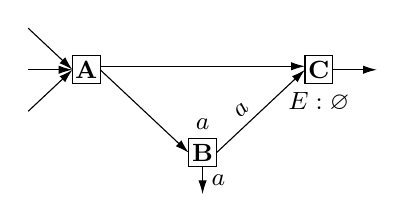
\begin{tikzpicture}[scale=1]
  
  \small
  
  \newcommand\X{210/5pt};
  \newcommand\Y{30pt};
  
  \draw[->] ( -0.5*\X, 0.5*\Y) -- ( -5+0*\X, 0*\Y);
  \draw[->] ( -0.5*\X, 0*\Y) -- ( -5+0*\X, 0*\Y);
  \draw[->] ( -0.5*\X, -0.5*\Y) -- ( -5+0*\X, 0*\Y);  

%  \draw[->] ( 5+2*\X, 0*\Y) -- ( 2.5*\X, 0.5*\Y);
  \draw[->] ( 5+2*\X, 0*\Y) -- ( 2.5*\X, 0*\Y);
%  \draw[->] ( 5+2*\X, 0*\Y) -- ( 2.5*\X, -0.5*\Y);  

%  \draw[->] ( 1*\X, -5-1*\Y) -- ( 1.5*\X, -1.5*\Y);
  \draw[->] ( 1*\X, -5-1*\Y) -- node[right]{$a$} ( 1*\X, -1.5*\Y);
%  \draw[->] ( 1*\X, -5-1*\Y) -- ( 0.5*\X, -1.5*\Y);  


  \draw[fill=white] (0*\X, 0*\Y) node{\textbf{A}} +(-5pt, -5pt) rectangle +(5pt, 5pt);
%  \draw (-5+0*\X, 0*\Y) node[left]{$E: \{a:2\}$};
  \draw[fill=white] (1*\X, -1*\Y) node{\textbf{B}} +(-5pt, -5pt) rectangle +(5pt, 5pt);
  \draw (1*\X, 5-1*\Y) node[above]{$a$};
  \draw[fill=white] (2*\X,  0*\Y) node{\textbf{C}} +(-5pt, -5pt) rectangle +(5pt, 5pt);
  \draw (2*\X, -5+0*\Y) node[below]{$E: \varnothing$};
%%  \draw (5+2*\X, 0*\Y) node[right]{\phantom{$E: \{a:1\}$}};

  \draw[->](5+0*\X, 0*\Y) -- (-5+1*\X, -1*\Y); %% A->B

  \draw[->](5+0*\X,  1.25+ 0*\Y) -- (-5+2*\X,  1.25+ 0*\Y); % A->C
 
  \draw[->](5+1*\X, -1*\Y) -- node[sloped, above]{$a\,\,\,\,\,\,$} (-5+2*\X, 0*\Y); %% B->C

\end{tikzpicture}}    
    \hspace{10pt}
    \subfloat[Part E][\label{fig:generalproblemE}Process~A broadcasts $a$. It expects 
    two copies of $a$.]
    {
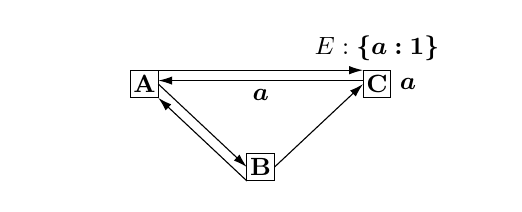
\begin{tikzpicture}[scale=1]
  
  \small
  
  \newcommand\X{210/5pt};
  \newcommand\Y{30pt};
  
  %% <spacing>
  \draw (-1*\X, 0);
  \draw (3*\X, 0);
  % </spacing>

  \draw[fill=white] (0*\X, 0*\Y) node{\textbf{A}} +(-5pt, -5pt) rectangle +(5pt, 5pt);
  % \draw (-5+0*\X, 0*\Y) node[left]{$E: \{a:2\}$};
  \draw[fill=white] (1*\X, -1*\Y) node{\textbf{B}} +(-5pt, -5pt) rectangle +(5pt, 5pt);
  % \draw (1*\X, -5-1*\Y) node[below]{$E: \varnothing$\vphantom{$\{$}};
  \draw[fill=white] (2*\X,  0*\Y) node{\textbf{C}} +(-5pt, -5pt) rectangle +(5pt, 5pt);
  \draw (2*\X, 5+0*\Y) node[above]{$E: \bm{\{a:1\}}$};%%$\vphantom{$\{$}};
  \draw (5+2*\X, 0*\Y) node[right]{$\bm{a}$};
  
  \draw[->](5+0*\X, 0*\Y) -- (-5+1*\X, -1*\Y); %% A->B
  \draw[<-](5+0*\X, -5+0*\Y) -- (-5+1*\X, -5-1*\Y); %% A<-B
  
  \draw[->](5+0*\X, 5+0*\Y) -- (-5+2*\X, 5+0*\Y); % A->C
  \draw[<-](5+0*\X,  1.25+ 0*\Y) -- node[below]{$\bm{a}$} (-5+2*\X,  1.25+ 0*\Y); % A<-C
  
  \draw[->](5+1*\X, -1*\Y) -- (-5+2*\X, 0*\Y); %% B<-C
  % \draw[->, dashed](5+1*\X, -5-1*\Y) -- (-5+2*\X, -5+0*\Y); %% B->C



\end{tikzpicture}}    
    \caption{Meow.}
  \end{center}
\end{figure*}


Unfortunately, such implementation does not handle dynamic systems where
processes can join, leave, or self-reconfigure their partial view at any
time. \TODO{Figure.} 

To solve this issue, state-of-the-art protocols maintain a local vector the size
of which increases linearly with the number of processes that ever broadcast a
message. They eventually become overcostly in dynamic settings.

In this paper, we exploit and extend \PCBROADCAST to provide a causal broadcast
middleware that is lightweight in terms of local memory consumption, and message
overhead. The next section describes the proposed protocol.

%%% Local Variables:
%%% mode: latex
%%% TeX-master: "../paper.tex"
%%% End:


\section{Issues and motivations (bis)}

Causal broadcast is a communication primitive that allows a process to send
messages to all processes of its distributed system (\REF). Message deliveries
follow the happen before relationship (\REF). If the sending of a message $m$
precedes the sending of a message $m'$ then all processes that deliver these two
messages need to deliver $m$ before $m'$. Otherwise they deliver them in any
order. Each process may receive a message multiple times but it delivers it
exactly once.


\begin{figure*}
  \begin{center}
    \subfloat[Part A][\label{fig:spaceproblemA}Process~B broadcasts $b$ along
    with control information $\langle B,\,1 \rangle$.]
    {\input{input/figspaceproblemA.tex}}
    \hspace{10pt}
    \subfloat[Part B][\label{fig:spaceproblemB}Process~A receives, saves in its
    local vector, delivers and forwards
    $b$. Process~B wants to add Process~C in its direct neighbors for
    causal broadcast. It sends a control message $\pi$ to Process~C using 
    Process~A as mediator.]
    {\input{input/figspaceproblemB.tex}}    
    \hspace{10pt}
    \subfloat[Part C][\label{fig:spaceproblemC}Process~A broadcasts $a$ along with
    control information $\langle A,\, 1 \rangle$. Then, it routes $\pi$ towards
    Process~C. Process~B receives $b$ but discards it, for it is already
    registered in Process~B's local vector.]
    {\input{input/figspaceproblemC.tex}}
    \hspace{10pt}
    \subfloat[Part D][\label{fig:spaceproblemD}Process~B and Process~C receive,
    save in their local vector, deliver and forward $a$. In addition, Process~B
    buffers $a$ to send it later to Process~C.]
    {\input{input/figspaceproblemD.tex}}
    \hspace{10pt}
    \subfloat[Part E][\label{fig:spaceproblemE}Process~C receives $\pi$ and 
    replies $\rho$ to Process~B.]
    {
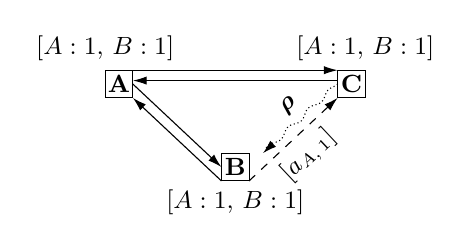
\begin{tikzpicture}[scale=1]
  
  \small
  
  \newcommand\X{210/5pt};
  \newcommand\Y{30pt};

  
  \draw[fill=white] (0*\X, 0*\Y) node{\textbf{A}} +(-5pt, -5pt) rectangle +(5pt, 5pt);
  \draw (-5+0*\X, 5+0*\Y) node[above]{$[A:1,\,B:1]$};
  \draw[fill=white] (1*\X, -1*\Y) node{\textbf{B}} +(-5pt, -5pt) rectangle +(5pt, 5pt);
  \draw (1*\X, -5-1*\Y) node[below]{$[A:1,\,B:1]$};
  \draw[fill=white] (2*\X,  0*\Y) node{\textbf{C}} +(-5pt, -5pt) rectangle +(5pt, 5pt);
  \draw (5+2*\X, 5+0*\Y) node[above]{$[A:1,\,B:1]$};
  
  \draw[->](5+0*\X, 0*\Y) -- 
  (-5+1*\X, -1*\Y); %% A->B

  \draw[<-](5+0*\X, -5+0*\Y) --
  (-5+1*\X, -5-1*\Y); %% A<-B
  
  \draw[->](5+0*\X, 5+0*\Y) --
  (-5+2*\X, 5+0*\Y); % A->C
  
  \draw[<-](5+0*\X,  1.25+ 0*\Y) --
  (-5+2*\X,  1.25+ 0*\Y); % A<-C
  
  % \draw[->,dashed](5+1*\X, -1*\Y) -- (-5+2*\X, 0*\Y); %% B<-C
 \draw[<-,densely dotted,decorate, decoration={snake, amplitude=0.3mm}](5+5+1*\X, 5+-1*\Y) -- 
 node[above, sloped]{$\bm{\rho}$}
 (-5+2*\X, 0*\Y);

  \draw[->, dashed](5+1*\X, -5-1*\Y) --
  node[sloped, below]{$[a_{A,\,1}]$} (-5+2*\X, -5+0*\Y); %% B->C



\end{tikzpicture}}
    \hspace{10pt}
    \subfloat[Part F][\label{fig:spaceproblemF}Process~B empties its buffer to
    Process~C. The latter will discard the message $a$, for it is already registered
    in Process~C's local vector]
    {\input{input/figspaceproblemF.tex}}

  \end{center}
\end{figure*}

%%% Local Variables:
%%% mode: latex
%%% TeX-master: "../paper"
%%% End:


\section{Proposal}
\label{sec:proposal}

In this section, we present \RPCBROADCAST, a causal broadcast protocol removing
the last linear upper bound in terms of number of processes that ever broadcast
a message that remained on space complexity. \RPCBROADCAST exploits the
improvement brought by \PCBROADCAST on generated traffic to reduce the space
consumed by reliable broadcast, at marginal cost.

\subsection{Model}

A distributed system comprises a set of processes that can communicate with each
other using messages. Processes may not have full knowledge of the membership of
the system. Instead, processes build and maintain overlay networks: each process
updates a local partial view of logical communication channels, i.e., a set of
processes to communicate with. The partial view is usually much smaller than the
actual system size. We speak of overlay networks, networks, or distributed
systems indifferently.

\begin{definition}[Overlay network]
  An overlay network comprises a set of processes that run a set of instructions
  sequentially.  An overlay network also comprises a set of directed
  links. \\
  An overlay network is dynamic if the set of processes and the set of links is
  mutable. Otherwise, the overlay network is static. \\
  The set of links departing from a process is its neighborhood, or partial
  view, or out-view. The set of links arriving to a process is its in-view. \\
  A link from a process to another process allows the former to transmit
  information to the latter. Processes transmit information using asynchronous
  message passing.\\
  Processes are faulty if they crash, otherwise they are correct. There are no
  byzantine processes.
\end{definition}

Processes can communicate with each other using message passing. Process~A can
send a message $m$ to Process~B $s_{AB}(m)$. Process~A can receive a message $m$
from another process B $r_{AB}(m)$, or from any other process
$r_A(m)$. Process~A can send a message $m$ to all other processes of the system,
i.e., it broadcasts a message $b_A(m)$. Process~A can deliver a message
$d_A(m)$.


\begin{definition}[Uniform reliable broadcast] 
  When a process broadcasts a message to all processes of the network, correct
  processes eventually receive it. Uniform reliable broadcast guarantees 3
  properties:
  \begin{itemize}
  \item Validity: If a correct process broadcasts a message, then it
    eventually delivers it.
  \item Uniform Agreement: If a process -- correct or not -- delivers a message,
    then all correct processes eventually deliver it.
  \item Uniform Integrity: A process delivers a message at most once, and only if
    it was previously broadcast.
  \end{itemize}
\end{definition}

\begin{algorithm}[h]
  \SetKwProg{Function}{function}{}{}
\SetKwProg{Upon}{upon}{}{}
\SetKwProg{Initially}{INITIALLY:}{}{}
\SetKwProg{Dissemination}{DISSEMINATION:}{}{}

\small

\DontPrintSemicolon
\LinesNumbered

\Initially {} {
  $Q_o$ \tcp*{Set of processes, $p$'s out-view}
  $Q_i$ \tcp*{Set of processes, $p$'s in-view}
  \BlankLine
  $E \leftarrow \varnothing$ \tcp*{Map of expected messages $Q_i : M^*$}
}

\BlankLine

\Dissemination{}{

%  \begin{multicols}{2}

  \Function{$\textup{R-broadcast}(m)$} { %\tcp*[f]{$b_p(m)$}} { 
    % $\textup{received}(m,\, \_)$ \;
    % \lForEach {$q \in Q_o$} {\textup{sendTo}($q,\, m$)}
    % \textup{R-deliver}($m$) \; % \tcp*{$d_p(m)$}
    $\textup{receive}(m,\, \_)$ \;
  }

  \BlankLine
  
  \Upon{$\textup{receive}(m,\, l)$}{
    \If {$\neg\textup{received}(m,\,l)$} {
      \lForEach {$q \in Q_o$} {\textup{sendTo}($q,\, m$)}
      % \tcp*[f]{broadcast or forward}}
      \textup{R-deliver}($m$) \; % \tcp*{$d_p(m)$}
    }
  }

  \BlankLine
  
  \Function{$\textup{received}(m,\, l)$}{
    \textbf{let} $rcvd \leftarrow
    \exists q \in E$ \textbf{\textup{with}} $m\in E[q]$ \;
    \If {$\neg rcvd$} {
      \ForEach {$q \in Q_i$} {$E[q] \leftarrow E[q] \cup m$ \label{line:remembers}}
        % \tcp*[f]{to remember}}
    }
    $E[l] \leftarrow E[l] \setminus m$ \label{line:forgets} \;%\tcp*{to forget}
    \Return $rcvd$ \;
  }

%  \end{multicols}

%  \BlankLine  
}


%%% Local Variables:
%%% mode: latex
%%% TeX-master: "../paper"
%%% End:

  \caption{\label{algo:reliablebroadcast}R-broadcast at Process $p$.}
\end{algorithm}

Algorithm~\ref{algo:reliablebroadcast} shows the instructions of a uniform
reliable broadcast that purges its local structure over time but only in static
networks. The implementation uses the in-view and exploits the property that
each process sends each message exactly once to each neighbor in their
out-view. It associates with each link from the in-view a set of awaited
messages. When Process~A receives a message for the first time from Process~B,
it awaits a copy of this message from all other processes in its in-view. Once
it receives this copy, it removes the message from the set of awaited
messages. Process~A will never receive a copy of this message from this
link. Once it received all awaited copies, it will never receive a copy of this
message. The principle of this implementation is similar to that of
Figure~\ref{fig:generalpurge} to which it adds an awareness of links with
awaited messages. Using this reliable broadcast implementation, each process
delivers each message exactly once.

In addition to reliable delivery, broadcast protocols can guarantee a delivery
order of messages. To define a delivery order among messages, we define time in
a logical sense using Lamport’s definition. 

\begin{definition}[Happen before~\cite{lamport1978time}]
  Happen before is a transitive, irreflexive, and antisymmetric relation that
  defines a strict partial orders of events. The sending of a message always
  precedes its receipt.
\end{definition}

\begin{definition}[Causal order]
  The delivery order of messages follows the happen before relationships of the
  corresponding broadcasts.
\end{definition}


\subsection{Operation}

Algorithm~\ref{algo:rpcbroadcast} shows the instructions of the proposed causal
broadcast. It relies on an implementation of reliable broadcast shown in
Algorithm~\ref{algo:reliablebroadcast}. When the process does not add links to
other processes, nor other processes add links to this process, causal broadcast
operation is that of reliable broadcast.

When the process wants to add a link to another process for causal broadcast, it
makes sure that this link cannot break the guaranty that the other process
delivers each message exactly once in causal order.


\begin{algorithm}[h]
  \SetKwProg{Function}{function}{}{}
\SetKwProg{Upon}{upon}{}{}
\SetKwProg{Initially}{INITIALLY:}{}{}
\SetKwProg{Safety}{SAFETY:}{}{}
\SetKwProg{Dissemination}{DISSEMINATION:}{}{}

\SetKwComment{EmptyComment}{}{}

\small

\DontPrintSemicolon
\LinesNumbered

%\begin{multicols}{2}
\Initially {} {
%  $Q_o$ \tcp*{Set of processes, $p$'s outview}
%  $Q_i$ \tcp*{Set of processes, $p$'s inview}
%  \BlankLine  
  $B \leftarrow \varnothing$ \tcp*{$@$Sender Map of buffers $Q_o : M^*$}
%  \BlankLine  
  $S \leftarrow \varnothing$ \tcp*{$@$Receiver Map of buffers $Q_i : M^* \times M^* \times bool$}
}

\BlankLine

\Dissemination{}{

  \begin{multicols}{2}
  \Function{$\RPCBROADCAST(m)$} { %\tcp*[f]{$b_p(m)$}} {
%    $\textup{buffering}(m)$ \;
    $\textup{R-broadcast}(m)$
  }

%  \BlankLine
  
  \Upon{$\textup{R-deliver}(m)$} {
    $\textup{buffering}(m)$ \;
    $\textup{PRC-deliver}(m)$
  }

%  \BlankLine

  \Function{$\textup{buffering}(m)$}{ 
    \lForEach {$q \in B$} {$B[q] \leftarrow B[q] \cup m$}

    \ForEach{$\langle B_\alpha,\, B_\pi,\, received_\pi\rangle \in S$}{
      \lIf{$received_\pi$}{$B_\pi \leftarrow B_\pi \cup m$}
      \lElse{$B_\alpha \leftarrow B_\alpha \cup m$}
    }
    
    %   $S[q] = \langle B_\alpha,\, \_,\, false \rangle$}
    % {$B_\alpha \leftarrow B_\alpha \cup m$}

    % \lForEach{$q \in S$ \textup{\textbf{such that}}
    %   $S[q] = \langle\, \_,\,B_\pi,\, true \rangle$}
    % {$B_\pi \leftarrow B_\pi \cup m$}

  }
  \end{multicols}
}

\BlankLine

\Safety{}{
  \begin{multicols}{2}
    \EmptyComment*[l]{\uline{$@$Sender}}
  \Upon{$\textup{open}_o(to)$} {
    $Q_o \leftarrow Q_o \setminus to$  \; % \tcp*{unsafe to send to $to$}
    $\textup{send-}\alpha(p,\,q)$ \label{line:sendalpha} \; %  \tcp*{$\alpha$}
  }

  \EmptyComment*[l]{\uline{$@$Receiver}}
  \Upon{$\textup{open}_i(from)$} {
    $Q_i \leftarrow Q_i \setminus from$ \; % \tcp*{unsafe to receive from $from$}
  }
  \end{multicols}

  \BlankLine
  
  \begin{multicols}{2}
  \Upon{$\textup{receive-}\beta(from,\,to)$}{% \tcp*[f]{$from=p$}} {
    $B[to] \leftarrow \varnothing$ \; %\tcp*{initialize $B_\beta$}
    $\textup{send-}\pi(from,\, to)$ \label{line:sendpi} \; % \tcp*{$\pi$}
  }

  \Upon{$\textup{receive-}\alpha(from,\,to)$}{ % \tcp*[f]{$to=p$}} {
    $S[from] \leftarrow \langle \varnothing,\, \varnothing,\, false \rangle$ \;
    %% \tcp*{initialize $B_\alpha$}
    $\textup{send-}\beta(from,\,to)$ \label{line:sendbeta} \; % \tcp*{$\beta$}
  }

  \end{multicols}
  
  \BlankLine
  
  \begin{multicols}{2}
  \Upon{$\textup{receive-}\rho(from,\,to)$}{% \tcp*[f]{$from=p$}} {
    $\textup{send-}B_\beta(from,\,to,\, B[to])$ \label{line:sendbuffer}\;
    $B \leftarrow B \setminus to$ \;
    $Q_o \leftarrow Q_o \cup to$ \; %\tcp*{safe to send to $to$}
  }

  \Upon{$\textup{receive-}\pi(from,\,to)$}{ % \tcp*[f]{$to=p$}} {
    \textbf{let} $\langle B_\alpha ,\, B_\pi ,\, \_ \rangle \leftarrow S[from]$ \;
    $S[from] \leftarrow \langle B_\alpha,\, B_\pi,\, true \rangle$ \; % \tcp*{initialize $B_\pi$}
    $\textup{send-}\rho(from,\, to)$ \label{line:sendrho} \; % \tcp*{$\rho$}
  }
  \end{multicols}

  \BlankLine
  
  \begin{multicols}{2}
    \EmptyComment*{}
    \EmptyComment*{}
    \EmptyComment*[r]{filter messages to ignore $\rightarrow$\hspace{2.2em}}
    \EmptyComment*[r]{to deliver $\rightarrow$\hspace{2.2em}}
    \EmptyComment*[r]{to expect $\rightarrow$\hspace{2.2em}}
    \columnbreak
  \Upon{$\textup{receive-}B_\beta(from,\, to,\, B_\beta)$} {
    \textbf{let} $\langle B_\alpha,\, B_\pi,\, \_ \rangle \leftarrow S[from]$ \;
%    \textbf{let} $potential \leftarrow buf \setminus B_\alpha$ \;
    \ForEach {$m \in B_\beta\setminus B_\alpha \setminus B_\pi$ }
    {$\textup{receive}(m,\,from)$ \label{line:todeliver}}  %$ \tcp*[f]{to deliver}}
    $E[from] \leftarrow B_\pi \setminus (B_\beta\setminus B_\alpha)$ \label{line:toexpect} \;% \tcp*{to expect}
    $S \leftarrow S \setminus from$ \;
    $Q_i \leftarrow Q_i \cup from$ \; % \tcp*{safe to receive from $from$}
  }
  \end{multicols}
  \BlankLine
  
  \begin{multicols}{2}
  \Upon{$\textup{close}_o(to)$} {
    $B \leftarrow B \setminus to$
  }
  \Upon{$\textup{close}_i(from)$} {
    $S \leftarrow S \setminus from$ \;
    $E \leftarrow E \setminus from$
  }
  \end{multicols}
  \BlankLine
}


%%% Local Variables:
%%% mode: latex
%%% TeX-master: "../paper"
%%% End:

  \caption{\label{algo:rpcbroadcast}RPC-broadcast at Process $p$.}
\end{algorithm}


\begin{figure*}
  \begin{center}
    \input{input/figtimelinerpcbroadcast.tex}
    \caption{Meow.}
  \end{center}
\end{figure*}

\subsection{Complexity}


%%% Local Variables:
%%% mode: latex
%%% TeX-master: "../paper"
%%% End:


\section{Experimentation}
\label{sec:experimentation}

\begin{figure*}
  \begin{center}
    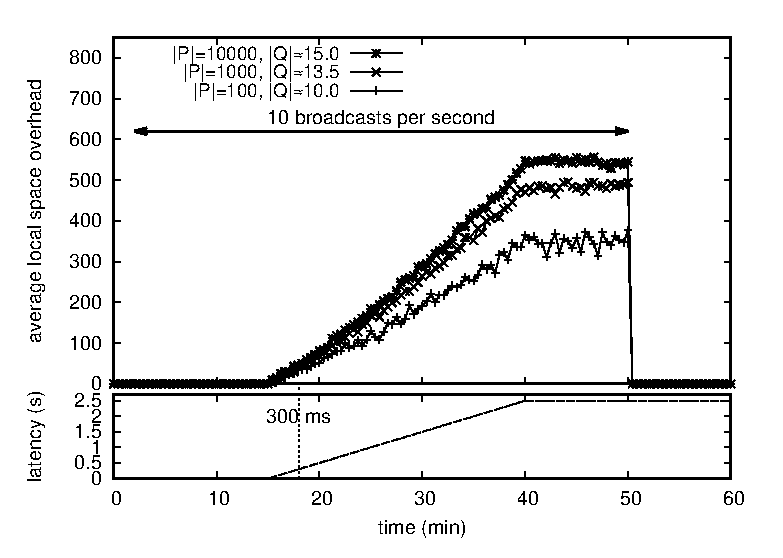
\includegraphics[width=0.65\textwidth]{./img/overhead.eps}
    \caption{\label{fig:overhead}Local space overhead over time consumed by
      \RPCBROADCAST to ensure causal order and forbid double delivery in dynamic
      systems with varying latency.}
  \end{center}
\end{figure*}


\RPCBROADCAST proposes a novel trade-off between speed, memory, and
traffic. Most importantly, its space consumed varies over receipts. In this
section, we evaluate the impact of the actual system on the space consumed and
traffic generated by processes. The experiments run on the \PEERSIM
simulator~\cite{montresor2009peersim} that allows to build large and dynamic
systems. Our implementation is available on the Github platform at
\url{http://github.com/chat-wane/peersim-prcbroadcast}.


% \begin{figure}
%   \begin{center}
%   
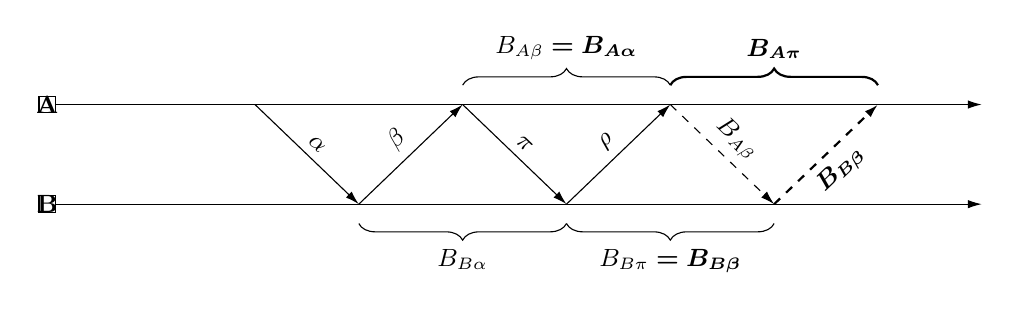
\begin{tikzpicture}[scale=0.6]

  \small
  
  \newcommand\X{1.45*\columnwidth/8pt};
  \newcommand\YA{0pt};
  \newcommand\YB{-60pt};


  \draw[->](0*\X, \YA) -- (9*\X, \YA);
  \draw[->](0*\X, \YB) -- (9*\X, \YB);
  
  \draw[fill=white] (0*\X, \YA) node{\textbf{\textup{A}}}
  +(-5pt, -5pt) rectangle +(5pt, 5pt);
  \draw[fill=white] (0*\X, \YB)  node{\textbf{\textup{B}}}
  +(-5pt, -5pt) rectangle +(5pt, 5pt);

  % \draw ( 1*\X, \YA ) node[above]{$\mathcal{A}$};
  % \draw ( 1*\X, \YB ) node[below]{$\mathcal{B}$};

  \draw[->] ( 2*\X, \YA ) -- node[sloped, above]{$\alpha$} (3*\X, \YB);
  % node[below left]{$\mathcal{A}$};

  \draw[decorate,decoration={brace,amplitude=6pt,mirror,raise=4pt}] (3*\X,
  -5+\YB) -- node[anchor=north, yshift=-10pt]{$B_{B\alpha}$}
  (5*\X, -5+\YB);

  % \draw ( 3*\X, \YA ) node[above]{$\mathcal{C}$};

  \draw[->] ( 3*\X, \YB ) -- node[sloped, above]{$\beta$} (4*\X, \YA);
  % node[above left]{$\mathcal{B}$};

  \draw[decorate,decoration={brace,amplitude=6pt,raise=4pt}] (4*\X,
  5+\YA) -- node[anchor=south, yshift=10pt]{$B_{A\beta} \bm{= B_{A\alpha}}$}
  (6*\X, 5+\YA);

  \draw[decorate,thick,decoration={brace,amplitude=6pt,raise=4pt}] (6*\X,
  5+\YA) -- node[anchor=south, yshift=10pt]{$\bm{B_{A\pi}}$}
  (8*\X, 5+\YA);
  
  
  % \draw ( 4*\X, \YB ) node[below]{$\mathcal{D}$};

  \draw[->] ( 4*\X, \YA ) -- node[sloped, above]{$\pi$} (5*\X, \YB);
  % node[below left]{$\mathcal{C}$};

  \draw[decorate,decoration={brace,amplitude=6pt,mirror,raise=4pt}] (5*\X,
  -5+\YB) -- node[anchor=north, yshift=-10pt]{$B_{B\pi} \bm{= B_{B\beta}}$}
  (7*\X, -5+\YB);


  % \draw ( 5*\X, \YA ) node[above]{$\mathcal{E}$};

  \draw[->] ( 5*\X, \YB ) -- node[sloped, above]{$\rho$} (6*\X, \YA);
  % node[above left]{$\mathcal{D}$};
  
  % \draw (6*\X, \YB) node[below]{$\mathcal{F}$};

  \draw[->, dashed] ( 6*\X, \YA ) -- node[sloped, above]{$B_{A\beta}$} (7*\X, \YB);

  \draw[->, dashed, thick] ( 7*\X, \YB ) --
  node[sloped, below]{$\bm{B_{B\beta}}$} (8*\X, \YA);

%  node[below left]{$\mathcal{E}$};


\end{tikzpicture}

%%% Local Variables:
%%% mode: latex
%%% TeX-master: "../paper"
%%% End:

%   \caption{\label{fig:bibroadcast}\RPCBROADCAST ensures the safety of bidirectional links
%     at marginal cost. Process~A maintains an additional buffer. Process~B transmits its
%     second buffer.}
%   \end{center}
% \end{figure}

\noindent \textbf{Objective:} To confirm that local space complexity
depends on in-views and message receipts.

\noindent \textbf{Description:} We measure the average size of buffers and
arrays of expected messages. This constitutes the average local space overhead
consumed by \RPCBROADCAST to detect and forbid multiple delivery in dynamic
systems.\\
Runs involve 3 overlay networks comprising 100, 1k, and 10k
processes. \SPRAY~\cite{nedelec2017adaptive} builds a highly dynamic overlay
networks that allows balancing the traffic generated by broadcasting among
processes. Each process maintains an out-view logarithmically scaling with the
number of processes in the system. Each process of the 100-processes system has
an out-view of $\approx 10$ neighbors. Each process of the 1k-processes system
has an out-view of $\approx 13.5$ neighbors. Each process of the 10k-processes
system has a out-view of $\approx 15$ neighbors. Each process dynamically
re-configures its out-view every minute by exchanging safe links with a chosen
neighbor: it gives half of its safe links to the chosen neighbor; the latter
gives half of its safe links to the former as well. Each exchange leads to link
memory initialization and safety checks of the new links,
and removal of given links.\\
Links are bidirectional, their safety must be checked in both directions but the
overhead remains minor. Links have transmission delay, i.e., the time between
the sending of a message and its receipt is not null. The experiments start with
$1$ millisecond transmission delay. At $15$ minutes, the delay starts to
increase. At $17$ minutes, links reach $300$ milliseconds transmission delay. At
$40$ minutes,
links reach $2.5$ seconds transmission delay and it stops increasing.\\
From $2$ minutes to $50$ minutes, every second, 10 processes chosen uniformly at
random among all processes broadcast a message.

\noindent \textbf{Results:} Figure~\ref{fig:overhead} shows the results of this
experiment. The x-axis denotes the time in minute. The top part of the figure
shows the local space overhead while the bottom part of the figure shows the
evolution of transmission delays.

\begin{figure*}
  \begin{center}
    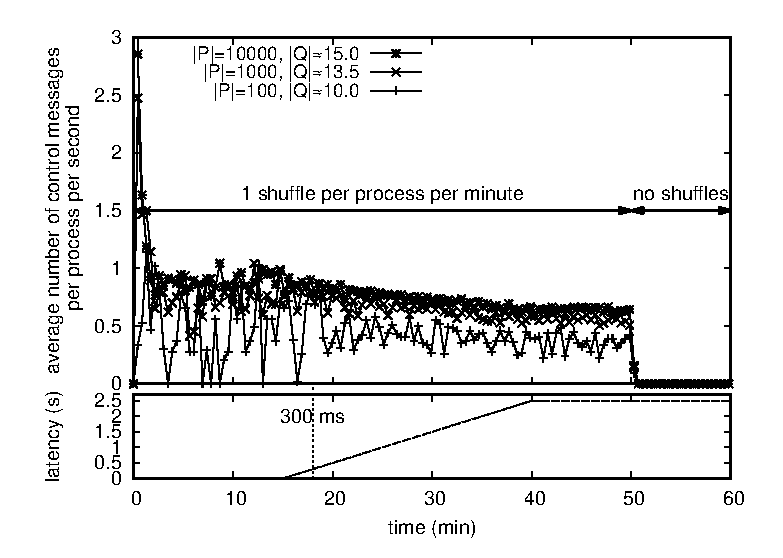
\includegraphics[width=0.65\textwidth]{./img/controlmessages.eps}
    \caption{\label{fig:controlmessages}Traffic overhead generated by
      \RPCBROADCAST.  Average number of control messages received --~including
      routing~-- per process for each second.}
  \end{center}
\end{figure*}



\begin{itemize}[leftmargin=*]
\item Figure~\ref{fig:overhead} confirms that the local space consumption
  depends on the in-view size. Systems with larger in-views consume more
  space. Each new delivered message adds control information on each link of the
  in-view (see Algorithm~\ref{algo:reliablebroadcast}).
\item Figure~\ref{fig:overhead} confirms that the local space consumption
  depends on network condition. The overhead increases as the latency
  increases. Latency increases the time between the first and the last receipt
  of each message. Processes store messages longer until they can be safely
  removed. 
\item Figure~\ref{fig:overhead} confirms that the local space consumption
  depends on broadcast messages. When processes stops broadcasting, the space
  consumed at each process drops to 0. Each process eventually receive each
  message and safely remove the corresponding entry.
\item Figure~\ref{fig:overhead} shows that at a rate of 10 broadcasts per second
  and when latency stays under a realistic bound ($300$ milliseconds), the overhead is
  lower than vector-based approaches. Whatever system conditions, it would
  require a vector of 100, 1k entries, 10k entries to forbid multiple delivery
  in the 100-processes system, 1k-processes system, 10k-processes system
  respectively. However, it is worth noting that the overhead of \RPCBROADCAST
  increases linearly with the number of messages currently transiting. 100
  broadcasts per second would multiply measurements made on \RPCBROADCAST by a
  factor of 10. In such case, the 100-entries vector would be better than
  \RPCBROADCAST even under a latency of $300$ milliseconds. 
\end{itemize}

\noindent \RPCBROADCAST provides a novel trade-off between speed, memory, and
traffic. Among other, its space consumed increases and decreases depending on
the system and its current use; instead of past use (see
Section~\ref{sec:relatedwork}. This result means that it constitutes an
advantageous trade-off in
\begin{inparaenum}[(i)]
\item dynamic systems
\item comprising up to millions of processes
\item that could broadcast at any time.
\end{inparaenum} \\

\noindent \textbf{Objective:} To confirm that the generated traffic overhead
depends on the dynamicity of the system.

\noindent \textbf{Description:} We measure the average number of control
messages received by each process during a second. This includes the routing of
messages. The setup is identical to that of prior experiment.

\noindent \textbf{Results:} Figure~\ref{fig:controlmessages} shows the results of
this experiment. The top part of the figure depicts the traffic overhead
generated by \RPCBROADCAST while the bottom part of the figure depicts the
evolution of transmission delays.

\begin{itemize}[leftmargin=*]
\item Figure~\ref{fig:controlmessages} shows that the number of control messages
  received by processes depends on the dynamicity of the system. The more
  dynamic the higher the traffic overhead. At the beginning of the experiment,
  processes join the system. Numerous links are established at once, hence the
  high number of control messages. Then processes shuffle their out-view during
  50 minutes. The number of links to add and remove is roughly constant over
  time, hence the stabilization in number of control messages. Finally,
  processes stop shuffling at $50$ minutes. Processes do not receive additional
  control messages.
\item Figure~\ref{fig:controlmessages} confirms our traffic overhead complexity
  analysis. For instance, in the 10k-processes system, views comprises 15
  processes which belong half from the out-view and half from the in-view.  Each
  process shuffles every minute. Each shuffle adds and removes 7.5 links (twice
  half of the out-view size). Since the peer-sampling protocol establishes links
  using neighbor-to-neighbor interactions, it allows a form of routing where
  only 8 control messages are required to initialize a new link.
  $|exchanged\_links|*|control\_messages|/60 \approx 7.5*8/60 \approx 1$ control
  message per second.
\item Figure~\ref{fig:controlmessages} shows that latency smooth and decreases
  the number of control messages. The peer-sampling protocol only shuffles links
  already safe and the memory of which is initialized. Since increasing latency
  increases the initialization time of links, processes exchange less links at
  each shuffle. The generated traffic decreases accordingly. Latency also
  spreads control messages over time, hence the smoothing in measurements.
\end{itemize}

% Overall, this section empirically confirms that the space complexity of
% \RPCBROADCAST is non-monotonic and depends on the system and its
% usage. Section~\ref{subsec:complexity} states that the space complexity is
% $O(Q_i.M)$ where $Q_i$ is the size of the in-view built by peer-sampling
% protocols, and $M$ is the number of messages that have been delivered but that
% will be received again. This experiment confirms that the space consumed by each
% process increases and decreases over time. In dynamic settings, this comes at
% the cost of control messages to initialize memory link.

\noindent Assuming peer-sampling protocols that enable a form of routing,
\RPCBROADCAST forbids multiple delivery at the cost of a few lightweight control
messages in dynamic systems. In this experiment, the underlying peer-sampling
protocol builds a random graph topology that has numerous desirable properties
such as resilience to failures, or load balancing~\cite{jelasity2007gossip}. It
fits dynamic systems where numerous processes join and leave
continuously. Nonetheless, other peer-sampling protocols could be used depending
on the configuration of the system. One could minimize latency using
Vivaldi~\cite{dabek2004vivaldi}, or gather people based on user preferences
using T-Man~\cite{jelasity2009tman}.


% However, it is worth noting that it remains in the hands of developers to choose
% the best peer-sampling protocol for their system (e.g. minimizing
% latency~\cite{dabek2004vivaldi}).


Overall, this section showed that \RPCBROADCAST proposes a novel trade-off in
terms of complexity. Its complexity actually depends on the system (its
dynamicity, its latency, its topology) and current use (broadcasts per second).
\RPCBROADCAST forbids multiple delivery and safely removes obsolete control
information about broadcast messages. The next section reviews state-of-the-art
approaches designed to forbid multiple delivery.




%%% Local Variables:
%%% mode: latex
%%% TeX-master: "../paper"
%%% End:


\section{Related Work}
\label{sec:relatedwork}

%%% Local Variables:
%%% mode: latex
%%% TeX-master: "../paper"
%%% End:


\section{Conclusion}
\label{sec:conclusion}


In this paper, we proposed an original causal broadcast protocol that removes
the last linear and monotonic upper bound that remained on local space
complexity. Our approach exploits causal order brought by causal broadcast to
improve the underlying reliable broadcast. The local space complexity depends on
the system and its usage. The overhead in terms of number of control messages
depends on the dynamicity of the system and remains low upon the assumption that
the overlay network allows a form of routing.
% Processes pay at the height of
% their usage.
% This approach only uses buffers of messages that grow and shrink when
% processes add new neighbors. They eventually become empty when the system
% becomes static. To achieve this, our approach only uses small control messages
% of constant size. The number of control messages depends on the overlay
% network. Using routing strategies, this number remains small, hence generated
% traffic overhead remains small.
This advantageous tradeoff makes causal broadcast a lightweight and efficient
middleware for group communication in distributed systems. This advantageous
tradeoff even makes \RPCBROADCAST a lightweight and efficient implementation for
reliable broadcast. %As consequence, causal broadcast and reliable broadcast can
%run in large and dynamic systems even on most humble devices such as Raspberry
%Pi’s.

As future work, we plan to investigate on ways to retrieve the partial order of
messages out of \RPCBROADCAST. Using \RPCBROADCAST, each process experiences a
flatten version of the partial order. However, several applications (\REF)
require more than causal order, they also need to identify concurrent
messages. \RPCBROADCAST discards a lot of information by ignoring multiple
receipts altogether. Analyzing the receipt order could provide insight on the
partial order. Instead of using vector clocks the cost of which increases with
the number of processes that ever broadcast, the cost could depend on the actual
concurrency of the system.

%%% Local Variables:
%%% mode: latex
%%% TeX-master: "../paper"
%%% End:


% \newpage

\section*{Acknowledgments}

This work was partially
funded by
% the French ANR project SocioPlug (ANR-13-INFR-0003), and by
% the DeSceNt project granted by the Labex CominLabs excellence laboratory
% (ANR-10-LABX-07-01).
the French ANR projects O'Browser (\mbox{ANR-16-CE25-0005-01}), and Descartes
(\mbox{ANR-16-CE40-0023}).

% Experiments presented in this paper were carried out using the Grid'5000
% testbed, supported by a scientific interest group hosted by Inria and including
% CNRS, RENATER and several Universities as well as other organizations (see
% \url{https://www.grid5000.fr}).

% \lipsum[56]

%%% Local Variables:
%%% mode: latex
%%% TeX-master: "../paper"
%%% End:


\bibliographystyle{plainurl}
\bibliography{bibliographie}
  
\end{document}

